\documentclass{beamer}
\usepackage[utf8]{inputenc}

\usepackage{minted}
\usepackage{pgf}
\usepackage{tikz}
\usepackage{upquote}
\usepackage{hyperref}
\usepackage{graphicx}
\usetikzlibrary{arrows,automata,positioning}

\setbeamertemplate{footline}[frame number]
\setbeamertemplate{navigation symbols}{}

\title{A Dependently-Typed Zipper over GADT-Embedded ASTs}
\author{Donovan Crichton}
\date{November 2018}

\begin{document}
 
\frame{\titlepage}

\begin{frame}[fragile]
  \frametitle{Preliminaries}
  \begin{itemize}
    \item \textbf{Slides and examples available at:}
    \url{https://github.com/donovancrichton/talkdepzip.git}
  \item \textbf{About me:}
    \begin{itemize}
      \item Honours 'year' student at Griffith University.
      \item Working towards a type-correct genetic program through
              dependently-typed functional programming.
      \item About 12 months experience in FP, just under 6 with
              dependent types.
    \end{itemize}
  \end{itemize}
\end{frame}

\begin{frame}[fragile]
  \frametitle{Acknowledgements}
  \begin{block}{A sincere thank you to..:}
    \begin{itemize}
      \item Mr Isaac Elliot (LightAndLight) (BFPG)
      \item Mr Alex Gryzlov (clayrat)
      \item The kind people from the Idris channel 
        on the discord functional programming server!
    \end{itemize}
  \end{block}
\end{frame}

\begin{frame}[fragile]
  \frametitle{A refresher on dependent types 1.}
  \begin{block}{A note on types and values.}
    \begin{itemize}
    \item Types can be functions and functions can be types!
    \item This takes some getting used to!
    \end{itemize}
  \end{block}
  \begin{minted}[fontsize=\small]{haskell}
  -- n is a value in the type signature
  -- n is also used as an argument to refer to that value.
  len : {a : Type} -> {n : Nat} -> Vec n a -> Nat
  len xs {n} = n
  \end{minted}
\end{frame}

\begin{frame}[fragile]
  \frametitle{A refresher on dependent types 2.}
  \begin{block}{A note on totality}
    \begin{itemize}
      \item Functions can be types.
      \item Functions need to be evaluated.
      \item We need a guarantee that our type-checker
        will eventually stop and give us a type.
      \item Any functions that are used as a type must be
        \textbf{total}!
      \item Total functions are defined for all cases and are guaranteed
        to terminate in some finite time.
    \end{itemize}
  \end{block}
\end{frame}

\begin{frame}[fragile]
\frametitle{A refresher on dependent types 3.}
\begin{itemize}
  \item The most basic definition is a dependent data type (GADT in
          Haskell).
  \item Dependent data types (DDT) depend on being parameterised over a
        type for their construction.
  \item Distinguished from parameterised ADTs by the ability to
        specify the return type parameter of each data constructor.
\end{itemize}
\begin{minipage}{0.5\textwidth}
\begin{block}{A vector dependent on a length value.}
\begin{minted}[fontsize=\small,baselinestretch=1]{haskell}
  data Nat = Z | S Nat

  data Vec : (n : Nat) -> (e : Type) -> Type where
    Nil : Vec Z e
    (::) : (x : e) -> (xs : Vec n e) -> Vec (S n) e
\end{minted}
\end{block}
\end{minipage}
\end{frame}

\begin{frame}[fragile]
  \frametitle{A refresher on dependent types 4.}

  \begin{block}{Why is this `good'?}
   If our length forms part of our type, we gain the ability
          to write correct functions with respect to vector length,
          without having to explicitly check. 
  \end{block}
  \begin{block}{Adding some vectors.}
  \begin{minted}[fontsize=\small]{haskell}
    -- Is this total? Defined for all cases and terminating?
    (+) : Num a => Vec n a -> Vec n a -> Vec n a
    (+) [] [] = []
    (+) (x :: xs) (y :: ys) = x + y :: xs + ys
  \end{minted}
  \end{block}
\end{frame}


\begin{frame}[fragile]
  \frametitle{A refresher on dependent types 5.}
  \begin{block}{$\Pi$ types.}
    \begin{itemize}
     \item The $\Pi$ type is a family of types that are indexed by a
           value (hence type families in Haskell).
     \item $\Pi$ types are used to calculate correct return types
             when given a specified value.
     \item In Idris $\Pi$ types only evaluate if the functions
             requiring them are marked as total.
     \item In Idris functions that return $\Pi$ types don't always
       evaluate in function composition, recursive calls or let bindings.
     \end{itemize}
  \end{block}
\end{frame}

\begin{frame}[fragile]
  \frametitle{A refresher on dependent types 6.}
  \begin{block}{An example of using $\Pi$ types in Idris.}
  \begin{minted}[fontsize=\small]{haskell}
  Age : Type
  Age = Nat

  Name : Type
  Name = String

  data Material = Plastic | Wood | Metal | Cheese
  data Person = P Name Age
  data Object = O Material

  IsPerson : Bool -> Type
  IsPerson True = Person
  IsPerson False = Object

  isPerson : (x : Bool) -> IsPerson x
  isPerson True = P "Donovan Crichton" 33
  isPerson False = O Cheese
  \end{minted}
  \end{block}
\end{frame}

\begin{frame}[fragile]
  \frametitle{A refresher on dependent types 7.}
  \begin{block}{$\Sigma$ types.}
  \begin{itemize}
    \item $\Sigma$ types are a pairing of a value, and a type that
            depends on that value (They are also called dependent
            pairs).
    \item $\Sigma$ types are useful when you want some basic type
            calculation around dependent types!
    \item Idris defines two functions for $\Sigma$ types:
          \mintinline{haskell}{fst} and \mintinline{haskell}{snd}
          for extracting the first and second elements of the pair.
          Similar to an ordinary product type (tuple).
  \end{itemize}
  \end{block}
\end{frame}

\begin{frame}[fragile]
  \frametitle{A refresher on dependent types 8.}
  \begin{block}{An example using $\Sigma$ types in Idris.}
  \begin{minted}[fontsize=\small]{haskell}
  data DPair : (a : Type) -> (P : a -> Type) -> Type where
    MkDPair : (x : a) -> (pf : P x) -> DPair a P

  -- also has some syntactic sugar in Idris.
  f : (x : Bool ** IsPerson x)
  f = (_ ** isPerson True)

  g : Num a => (n : Nat ** Vec n a)
  g = (_ ** [1, 2, 3])

  -- this is particularly useful if we are passing a vector
  -- of unknown length in as an argument.
  len : Num a => Vec n a -> (x : Nat ** Vec x a)
  len x = (_ ** x)

  -- len [1, 2, 3] returns
  -- (3 ** [1, 2, 3]) : (x : Nat ** Vec x Integer)
  \end{minted}
  \end{block}
\end{frame}

\begin{frame}[fragile]
  \frametitle{A refresher on dependent types 9.}
  \begin{block}{The Curry-Howard Isomorphsim.}
  The CH Isomorphsim shows the relationship between mathematical
    proofs under logic, and computer programs. In Idris this
    relationship can be expressed as follows:
  \begin{table}[h!]
    \begin{tabular}{c|c|c|c}
    \textbf{Logic Term} & \textbf{Logic Symbol} & \textbf{Idris Symbol}
      & \textbf{Idris Type} \\
    \hline
      Implication & p $\Rightarrow$ q & p \mintinline{haskell}{->} q
      & Arrow \\
      Conjunction & p $\land$ q & \mintinline{haskell}{(p, q)} 
      & Pair (Product) \\
      Disjunction & p $\lor$ q & \mintinline{haskell}{Either p q}
      & Enum (Sum)\\
      Negation & $\lnot$ p & \mintinline{haskell}{p -> Void} &
      Void Type \\
      IFF/Eq & p $\equiv$ q, p $\iff$ q & \mintinline{haskell}{(p -> q, q -> p)}
      & Pair Arrows \\
      Universal & $\forall$ x. P x & 
      \mintinline{haskell}{p -> Type} & $\Pi$ Type \\
      Existential & $\exists$ x. P x
      & \mintinline{haskell}{(x ** P x)} & $\Sigma$ Type \\
      \hline
      ??? & ??? & \mintinline{haskell}{p = q} & Type Equality
    \end{tabular}
    
  \end{table}
  \end{block}
\end{frame}

\begin{frame}[fragile]
  \frametitle{A refresher on dependent types 9.}
  \begin{block}{Why are $\Sigma$ and $\Pi$ `good'?}
  \begin{itemize}
    \item $\Pi$ types let us map types to values.
    \item We can now be more precise about function values.
    \item $\Sigma$ types let us specify properties of types, even
      when we may not know the exact return type at compile time.
    \item `properties' includes both $\Pi$ types, and types that are
      parameterised over other types.
    \item This will become much clearer later!
  \end{itemize}
  \end{block}
\end{frame}

\begin{frame}[fragile]
  \frametitle{Motivation}
  \begin{itemize}
    \item Came from a research project on the automatic generation of 
      well-typed functions to solve a given problem.
    \item We'd like to substitute values at specific positions on
      the expression tree.
    \item We may not know the value at the position during run-time
      (but we may know its type).
    \item A zipper allows the specification of a position in a tree
      via a path of transformations or rotations.
    \item We'd like to exchange values of the same type at different
      positions between two trees.
  \end{itemize}
\end{frame}

\begin{frame}[fragile]
  \frametitle{Dependent data type embedded DSLs 1.}
  \begin{block}{A quick review of DSLs}
    \begin{itemize}
      \item Short for Domain Specific Language.
      \item Used in lots of places, salary calculations, query and
        markup languages, business logic, etc.
    \end{itemize}
  \end{block}
  \begin{block}{A DDT (or GADT) embedded DSL}
    \begin{minted}[fontsize=\small]{haskell}
      data Expr : (a : Type) -> Type where
        Lit   : a -> Expr a
        Add   : Num a => Expr a -> Expr a -> Expr a
        Const : Expr a -> Expr b -> Expr a
    \end{minted}
  \end{block}
\end{frame}

\begin{frame}[fragile]
  \frametitle{Dependent data type embedded DSLs 2.}
  \begin{block}{An embedded DSL and it's interpreter.}
    \begin{minted}[fontsize=\small]{haskell}
      data Expr : (a : Type) -> Type where
        Lit   : a -> Expr a
        Add   : Num a => Expr a -> Expr a -> Expr a
        Const : Expr a -> Expr b -> Expr a

      interp : Expr a -> a
      interp (Lit x)     = x
      interp (Add x y)   = (interp x) + (interp y)
      interp (Const x y) = const (interp x) (interp y)
    \end{minted}
  \end{block}
  \begin{block}{Why is an embedded DSL `good'?}
    \begin{itemize}
      \item It was very easy to write that interpreter.
      \item The type checker over the meta language takes care of
        type checking the DSL.
      \item The meta language also takes care of variable binding.
    \end{itemize}
  \end{block}
\end{frame}

\begin{frame}[fragile]
  \frametitle{Dependent data type embedded DSLs 3.}
  \begin{block}{Expressions as Trees}
  \mintinline{haskell}{Const (Add (Lit 2) (Lit 3)) (Lit "Test"))}
  \begin{center}
    \begin{tikzpicture}
      \node[shape=circle, draw=black, minimum size = 1.5cm] (Exp) {Const} ;
      \node[shape=circle, draw=black, minimum size = 1.5cm] (Add) 
           [below left = 2cm of Exp] {$+$};
      \node[shape=circle, draw=black, minimum size = 1.5cm] (2) 
           [below left = 2cm of Add] {2};
      \node[shape=circle, draw=black, minimum size = 1.5cm] (3)
           [below right = 2cm of Add] {3};
      \node[shape=circle, draw=black, minimum size = 1.5cm] (Test)
           [below right = 2cm of Exp] {``Test''};

      \path [-] (Exp) edge node {} (Add);
      \path [-] (Exp) edge node {} (Test);
      \path [-] (Add) edge node {} (2);
      \path [-] (Add) edge node {} (3);
     \end{tikzpicture}
  \end{center}
  \end{block}
\end{frame}

\begin{frame}[fragile]
  \frametitle{Zipping over embedded DSLs LYAH style (Naive).}
    \begin{minted}[fontsize=\small]{haskell}
      data Expr : Type -> Type where
        Lit   : a -> Expr a
        Add   : Num a => Expr a -> Expr a -> Expr a
        Const : Expr a -> Expr b -> Expr a

      data Context = Root
        | L (Expr a) Context
        | R (Expr a) Context

      left : (Expr a, Context) -> (Expr a, Context)
      left (Lit x, c)     = (Lit x, c)
      left (Add x y, c)   = (x, L (Add x y) c)
      left (Const x y, c) = (x, L (Const x y) c)

      -- the problem comes when trying to write right
      right : (Expr a, Context) -> (Expr a, Context)
      right (Lit x, c)     = (Lit x, c)
      right (Add x y, c)   = (y, R (Add x y) c)
      right (Const x y, c) = (y, R (Const x y) c)
    \end{minted}
\end{frame}

\begin{frame}[fragile]
  \frametitle{Zipper over embedded DSLs LYAH style 2 (Naive).}
  \begin{block}{Why doesn't this work?}
    \begin{itemize}
      \item `left' works fine because the compiler can see
        that all instances of left result in an `Expr a'.
      \item `right' cannot type-check because the compiler
        sees that it returns an `Expr b' in the `Const' case.
    \end{itemize}
  \end{block}
  \begin{block}{Where to from here?}
    \begin{itemize}
      \item There is nothing stopping us from writing a nonsensical
        context and pairing it up with some expression. We'd like 
        some stronger guarantees here.
      \item Lets try to get some stronger intuition of what needs to happen!
      \item Lets also see how far we can get with dependent types!
    \end{itemize}
  \end{block}
\end{frame}

\begin{frame}[fragile]
  \frametitle{Some Intuition.}
  \begin{block}{Going right down the expression tree.}
  \mintinline{haskell}{Const (Add (Lit 2) (Lit 3)) (Lit "Test")} \\
  Let C represent Const. Let T represent ``Test''. \\
  \end{block}
  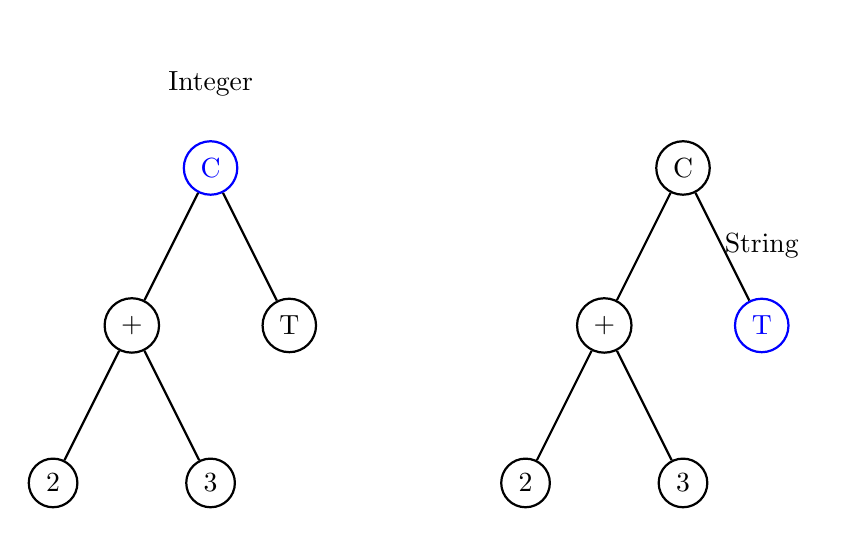
\begin{tikzpicture}
    %Tree 1
     \begin{scope}[every node/.style={circle,thick,draw}]
       \node[label={Integer}, draw=blue, text=blue] (const) at (-6,0) {C};
       \node (add) at (-7,-2) {+};
       \node (test) at (-5,-2) {T};
       \node (2) at (-8,-4) {2};
       \node (3) at (-6,-4) {3};
    \end{scope}

    \begin{scope}[every edge/.style={draw,thick, circle},
       every node/.style={circle}]
      \path (const) edge (add);
      \path (const) edge (test);
      \path (add) edge (2);
      \path (add) edge (3);
    \end{scope}

    %Tree 2
     \begin{scope}[every node/.style={circle,thick,draw}]
       \node (const) at (0,0) {C};
       \node (add) at (-1,-2) {+};
       \node[label={String},text=blue, draw=blue] (test) at (1,-2) {T};
       \node (2) at (-2,-4) {2};
       \node (3) at (0,-4) {3};
    \end{scope}

    \begin{scope}[every edge/.style={draw,thick, circle},
       every node/.style={circle}]
      \path (const) edge (add);
      \path (const) edge (test);
      \path (add) edge (2);
      \path (add) edge (3);
    \end{scope}
  \end{tikzpicture}
\end{frame}

\begin{frame}[fragile]
  \frametitle{More Intuition.}
  \begin{block}{Going left down the expression tree.}
  \mintinline{haskell}{Const (Add (Lit 2) (Lit 3)) (Lit "Test")} \\
  Let C represent Const. Let T represent ``Test''. \\
  \end{block}
  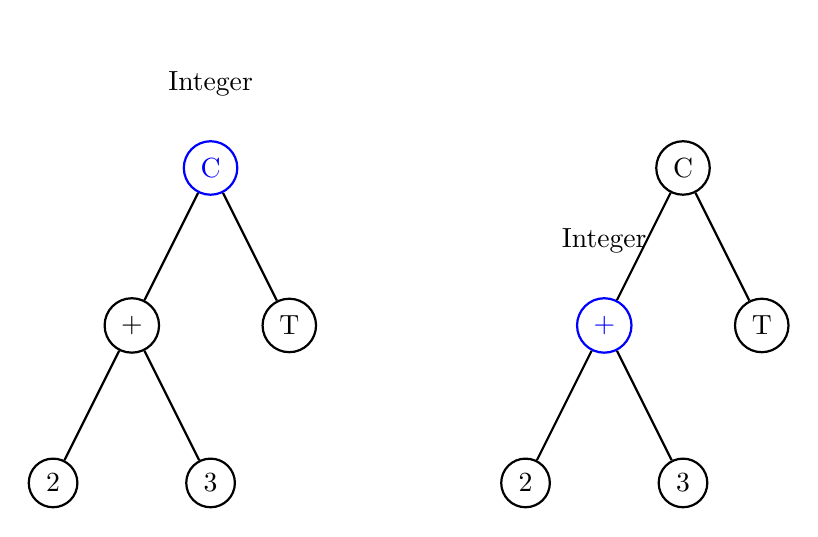
\begin{tikzpicture}
    %Tree 1
     \begin{scope}[every node/.style={circle,thick,draw}]
       \node[label={Integer}, draw=blue, text=blue] (const) at (-6,0) {C};
       \node (add) at (-7,-2) {+};
       \node (test) at (-5,-2) {T};
       \node (2) at (-8,-4) {2};
       \node (3) at (-6,-4) {3};
    \end{scope}

    \begin{scope}[every edge/.style={draw,thick, circle},
       every node/.style={circle}]
      \path (const) edge (add);
      \path (const) edge (test);
      \path (add) edge (2);
      \path (add) edge (3);
    \end{scope}

    %Tree 2
     \begin{scope}[every node/.style={circle,thick,draw}]
       \node (const) at (0,0) {C};
       \node[label={Integer}, draw=blue, text=blue] (add) at (-1,-2) {+};
       \node (test) at (1,-2) {T};
       \node (2) at (-2,-4) {2};
       \node (3) at (0,-4) {3};
    \end{scope}

    \begin{scope}[every edge/.style={draw,thick, circle},
       every node/.style={circle}]
      \path (const) edge (add);
      \path (const) edge (test);
      \path (add) edge (2);
      \path (add) edge (3);
    \end{scope}
  \end{tikzpicture}
\end{frame}
\begin{frame}[fragile]
  \frametitle{A dependently typed zipper 1.}
  \begin{block}{Let's start with $\Pi$ types.}
    \begin{itemize}
    \item These $\Pi$ types will allow us to calculate the correct type
          of the context, and keep us honest when developing the zipper.
    \item Have a look at the `Maybe Type`. It doesn't make sense for us to
          build a type from going left or right on the `Lit x' case.
    \end{itemize}
    \begin{minted}[fontsize=\small]{haskell}
      GoLeft : Expr a -> Maybe Type
      GoLeft (Lit x) = Nothing
      GoLeft (Add {a} x y) = Just a
      GoLeft (Const {a} x y) = Just a

      GoRight : Expr a -> Maybe Type
      GoRight (Lit x) = Nothing
      GoRight (Add {a} x y) = Just a
      GoRight (Const {b} x y) = Just b
    \end{minted}
  \end{block}
\end{frame}

\begin{frame}[fragile]
  \frametitle{A dependently typed zipper 2.}
  \begin{block}{Let's re-define the context.}
    \begin{itemize}
      \item By parameterising the context over our $\Pi$ types, we
        ensure that the type checker will fail when we try to build
        invalid contexts.
      \item Moving from an ADT to a DDT (GADT) gives us a lot more
        expressivity here! This is also a strong example of the
        dependence relationship in the type parameter.
    \end{itemize}
    \begin{minted}[fontsize=\small]{haskell}
data Context : Maybe Type -> Type where
  Root : Context (Just a)
  L : (x : Expr a) -> Context (Just a) -> Context (GoLeft x)
  R : (x : Expr a) -> Context (Just a) -> Context (GoRight x)
    \end{minted}
  \end{block}
\end{frame}

\begin{frame}[fragile]
  \frametitle{A dependently typed zipper 3.}
  \begin{block}{Let's re-define the zipper.}
    \begin{itemize}
      \item We'd like to parameterise the zipper so that we can
        perform operations on zippers that have holes (or focii) of
        the same type.
      \item `wrap' is provided to give us an easy way of creating a
        $\Sigma$ type from a zipper, we wrap all this up in a `Maybe'
        as some zipping operations may fail.
    \end{itemize}
  \begin{minted}[fontsize=\small]{haskell}
data Zipper : Type -> Type where
  Zip : Expr a -> Context (Just a) -> Zipper a

wrap : Zipper a -> Maybe (a : Type ** Zipper a)
wrap x = Just (_ ** x)
  \end{minted}
  \end{block}
\end{frame}

\begin{frame}[fragile]
  \frametitle{A dependently typed zipper 4.}
  \begin{block}{Re-defining the direction functions.}
    \begin{minted}[fontsize=\small]{haskell}
left : Maybe (a : Type ** Zipper a) 
    -> Maybe (b : Type ** Zipper b)
left Nothing = Nothing
left (Just (x ** pf)) = 
  case pf of
    (Zip p@(Lit x) c) => Nothing
    (Zip p@(Add x y) c) => Just (_ ** Zip x (L p c)) 
    (Zip p@(Const x y) c) => Just (_ ** Zip x (L p c)) 

right : Maybe (a : Type ** Zipper a) 
     -> Maybe (b : Type ** Zipper b)
right Nothing = Nothing
right (Just (x ** pf)) = 
  case pf of
    (Zip p@(Lit x) c) => Nothing 
    (Zip p@(Add x y) c) => Just (_ ** Zip y (R p c)) 
    (Zip p@(Const x y) c) => Just (_ ** Zip y (R p c)) 
     \end{minted}
  \end{block}
\end{frame}

\begin{frame}[fragile]
  \frametitle{A dependently typed zipper 5.}
  \begin{block}{Notes on the left and right directions.}
    \begin{itemize}
      \item Thanks to the `GoLeft' and `GoRight' $\Pi$ types 
        we defined earlier. It's not possible to accidentally
        produce a focus of the incorrect type when implementing
        `left' and `right'.
      \item We can say that the type is now correct by construction.
    \end{itemize}
  \end{block}
\end{frame}

\begin{frame}[fragile]
  \frametitle{A dependently typed zipper 6.}
  \begin{block}{Gotchas in the context?}
    \begin{itemize}
      \item Do we need to store the full parent expression?
      \item Can we get away with returning a partially applied function?
      \item What would we gain or lose? There is more to think about!
      \item The left and right constructors are used in the next direction
        case.
    \end{itemize}
  \end{block}
\end{frame}

\begin{frame}[fragile]
  \frametitle{A dependently typed zipper 7.}
  \begin{block}{More direction functions.}
    \begin{minted}[fontsize=\small]{haskell}
up : Maybe (a : Type ** Zipper a) 
  -> Maybe (b : Type ** Zipper b)
up Nothing = Nothing
up (Just (x ** pf)) =
 case pf of
  (Zip e Root) => Just (_ ** Zip e Root)
  (Zip e (R (Lit x) pc)) impossible
  (Zip e (R (Add x y) pc)) => Just (_ ** Zip (Add x e) pc)
  (Zip e (R (Const x y) pc)) => Just (_ ** Zip (Const x e) pc)
  (Zip e (L (Lit x) pc)) impossible
  (Zip e (L (Add x y) pc)) => Just (_ ** Zip (Add e y) pc)
  (Zip e (L (Const x y) pc)) => Just (_ ** Zip (Const e y) pc)
    \end{minted}
  \end{block}
\end{frame}

\begin{frame}[fragile]
  \frametitle{A dependently typed zipper 8.}
  \begin{block}{\mintinline{haskell}{up} and $\Sigma$ types.}
    \begin{itemize}
      \item Remember, we say a function is total when it is defined
        for all cases and is guaranteed to terminate in finite time.
      \item $\Pi$ and $\Sigma$ types do not refine if used to define
        non-total functions in Idris.
      \item To make `up' total, we must list all the cases!
      \item Some cases are clearly nonsense though!
      \item We can mark those as impossible in Idris to keep the
        function total.
    \end{itemize}
  \end{block}
\end{frame}

\begin{frame}[fragile]
  \frametitle{A dependently typed zipper 9.}
  \begin{block}{A graphical representation of `subst'}
  \mintinline{haskell}{Const (Add (Lit 2) (Lit 3)) (Lit "Test")}
  Let C represent Const.
  Let T represent "Test'. Let H represent "Hello".
  \end{block}
  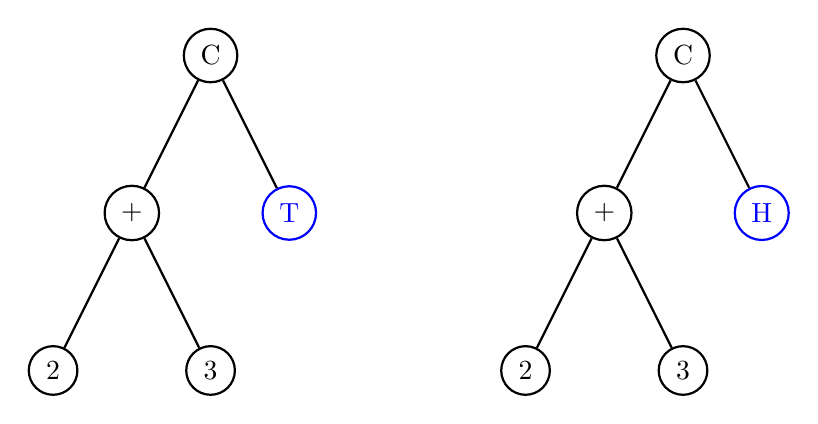
\begin{tikzpicture}
    %Tree 1
     \begin{scope}[every node/.style={circle,thick,draw}]
       \node (const) at (-6,0) {C};
       \node (add) at (-7,-2) {+};
       \node[draw=blue,text=blue] (test) at (-5,-2) {T};
       \node (2) at (-8,-4) {2};
       \node (3) at (-6,-4) {3};
    \end{scope}

    \begin{scope}[every edge/.style={draw,thick, circle},
       every node/.style={circle}]
      \path (const) edge (add);
      \path (const) edge (test);
      \path (add) edge (2);
      \path (add) edge (3);
    \end{scope}

    %Tree 2
     \begin{scope}[every node/.style={circle,thick,draw}]
       \node (const) at (0,0) {C};
       \node (add) at (-1,-2) {+};
       \node[draw=blue,text=blue] (test) at (1,-2) {H};
       \node (2) at (-2,-4) {2};
       \node (3) at (0,-4) {3};
    \end{scope}

    \begin{scope}[every edge/.style={draw,thick, circle},
       every node/.style={circle}]
      \path (const) edge (add);
      \path (const) edge (test);
      \path (add) edge (2);
      \path (add) edge (3);
    \end{scope}
  \end{tikzpicture}
\end{frame}

\begin{frame}[fragile]
  \frametitle{A dependently typed zipper 9.}
  \begin{block}{Substitution and evaluation.}
  \begin{minted}[fontsize=\small]{haskell}
subst : (x : (a : Type ** Zipper a)) 
       -> Expr (fst x) 
       -> Maybe (b : Type ** Zipper b)
subst (x ** (Zip x' c)) e = Just (_ ** Zip e c)

data NotNothing : Maybe a -> Type where
  IsNotNothing : NotNothing (Just x)

fromMaybe : (input : Maybe (a : Type ** Zipper a))
           -> {auto prf : NotNothing input}
           -> (a : Type ** Zipper a)
fromMaybe (Just z) = z

interp : (x : (a : Type ** Zipper a)) -> (fst x)
interp (x ** (Zip e c)) = eval e
  \end{minted}
  \end{block}
\end{frame}

%\begin{frame}[fragile]
%  \frametitle{A dependently typed zipper 10.}
%  \begin{block}{Notes on substitution, interpretation and `Just' proofs.}
%    \begin{itemize}
%      \item We write `subst' under the assumption that we have an ordinary
%        $\Sigma$ type parameterised by `a' and a further expression also
%        parameterised by `fst x'. This ensures that the function will calculate
%        the correct type!
%      \item We defined `NotNothing' and `fromMaybe' to give us some tools
%        to access the underlying type parameter. We can also achieve this
%        with more $\Sigma$ types.
%    \end{itemize}
%  \end{block}
%\end{frame}

\begin{frame}[fragile]
  \frametitle{But...does it actually work?}
  \begin{minted}[fontsize=\small]{haskell}
ex1 : Num a => Zipper a
ex1 = Zip (Const (Lit 2) (Lit "Test")) Root
-- Zip (Const (Lit 2) (Lit "Test")) Root

ex2 : Maybe (a : Type ** Zipper a)
ex2 = wrap ex1
-- Just (Integer ** Zip (Const (Lit 2) (Lit "Test")) Root)

ex3 : Maybe (a : Type ** Zipper a)
ex3 = right ex2
-- Just (String ** 
--   Zip (Lit "Test") (R (Const (Lit 2) (Lit "Test")) Root))

ex4 : Maybe (a : Type ** Zipper a)
ex4 = up (subst (fromMaybe ex3) (Lit "Hello"))
-- Just (Integer ** Zip (Const (Lit 2) (Lit "Hello")) Root)

ex5 : (DPair.fst (fromMaybe Main.ex4))
ex5 = interp (fromMaybe ex4)
-- 2
  \end{minted}
\end{frame}

\begin{frame}[fragile]
  \frametitle{Gotchas! (Further work).}
  \begin{itemize}
    \item The $\Sigma$ type \mintinline{haskell}{Maybe (a : Type ** Zipper a)}
      is not really idiomatic.
    \item It's more correct to have 
      \mintinline{haskell}{(a : Type ** Zipper a ** Maybe (Zipper a))}
    \item This is more cumbersome in some ways to work with, and harder to
      grasp if unfamiliar with $\Sigma$ types.
    \item How necessary is it to parameterise the context over a `Maybe Type'?
    \item This is in no way generic! Our zipping functions, and our context
      are both tightly coupled to the structure of our DSL. 
  \end{itemize}
\end{frame}

\begin{frame}[fragile]
  \frametitle{In summary.}
  \begin{itemize}
    \item We've shown the implementation of a method to correctly traverse a
      DDT-embedded DSL, where the types can be calculated at run-time.
    \item This is working towards the automated generation of well-typed
      expressions.
    \item Dependent types allow us to use our type-checker as a proof-checker.
    \item Dependent types also allow us to reduce the number of invalid
      programs.
  \end{itemize}
\end{frame}

\begin{frame}[fragile]
  \frametitle{Resources.}
  \begin{block}{Dependent Types}
    \begin{itemize}
      \item B-trees with GADTS by Matthew Brecknel: 
        https://www.youtube.com/watch?v=VIeZW4TSSHg (Talk)
      \item Type-Driven Development with Idris - Edwin Brady (Book).
      \item The Little Typer - Daniel P. Friedman and David Thrane Christiansen
        (Book).
    \end{itemize}
  \end{block}
  \begin{block}{Curry Howard Isomorphsim}
    \begin{itemize}
      \item Propositions as Types - Phillip Wadler (Paper).
    \end{itemize}
  \end{block}
  \begin{block}{Theorem Proving with Dependent Types}
    \begin{itemize}
      \item Software Foundations 
        https://softwarefoundations.cis.upenn.edu/
        (Book Series)
    \end{itemize}
  \end{block}
\end{frame}

\end{document}
